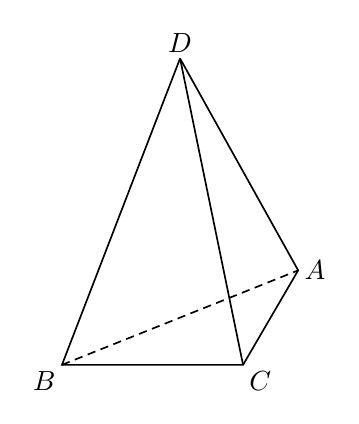
\begin{tikzpicture}[line width=.6pt,font=\normalsize,inner sep=2pt]
\coordinate (A) at (1.5000000000,0.6000000000);
\coordinate (B) at (-1.5000000000,-0.6000000000);
\coordinate (C) at (0.8000000000,-0.6000000000);
\coordinate (D) at (0.0000000000,3.2908965344);
\draw (D)--(B)--(C)--(A)--(D);
\draw (D)--(C);
\draw[densely dashed] (B)--(A);
\node[right] at (A) {$A$};
\node[below left] at (B) {$B$};
\node[below right] at (C) {$C$};
\node[above] at (D) {$D$};
\end{tikzpicture}
